\documentclass[12pt,a4paper]{article}

%These cannot go before lwarp!
%\usepackage{hyperref} %This one warns us
%\usepackage{graphicx} %This one doesn't

%This will not be accessible as the maths will be images...
\usepackage{lwarp}
%\usepackage[mathjax]{lwarp}
%\usepackage[
%   HomeHTMLFilename=index,     % Filename of the homepage.
%   HTMLFilename={part-},       % Filename prefix of other pages.
%   mathjax                     % Use MathJax to display math.
%]{lwarp}
%\setcounter{FileDepth}{2}      % Split HTML files at sections
%\setcounter{SideTOCDepth}{2}   % Include subsections in the side TOC

\usepackage{hyperref}
\usepackage{graphicx}
\usepackage{amsmath,amssymb}
\usepackage[margin=2.5cm]{geometry}

\setlength{\parindent}{0.0pt}

\newcommand{\RR}{\mathbb{R}}
%Without the below the command will not work in mathjax
%\begin{warpHTML}
%\CustomizeMathJax{\newcommand{\RR}{\mathbb{R}}}
%\end{warpHTML}

\title{Example}
\author{Emma Cliffe}
\date{2022}

\HTMLAuthor{Emma Cliffe}       % Sets the HTML meta author tag.
\HTMLLanguage{en-UK}             % Sets the HTML meta language.
\HTMLDescription{First example of using Lwarp}% Sets the HTML meta description.

\begin{document}
\maketitle

\tableofcontents

\section{Arc length}

We often need to know the length of a curve between two points,
e.g.~what is the length of the ropes holding Clifton suspension bridge
(see Exercise Sheet 3).

\subsection{Visualisation}

Given the curve \(y=y(x), x \in \RR\), illustrated in figure \ref{arclength1}.

\begin{figure}[!hptb]
\begin{center}
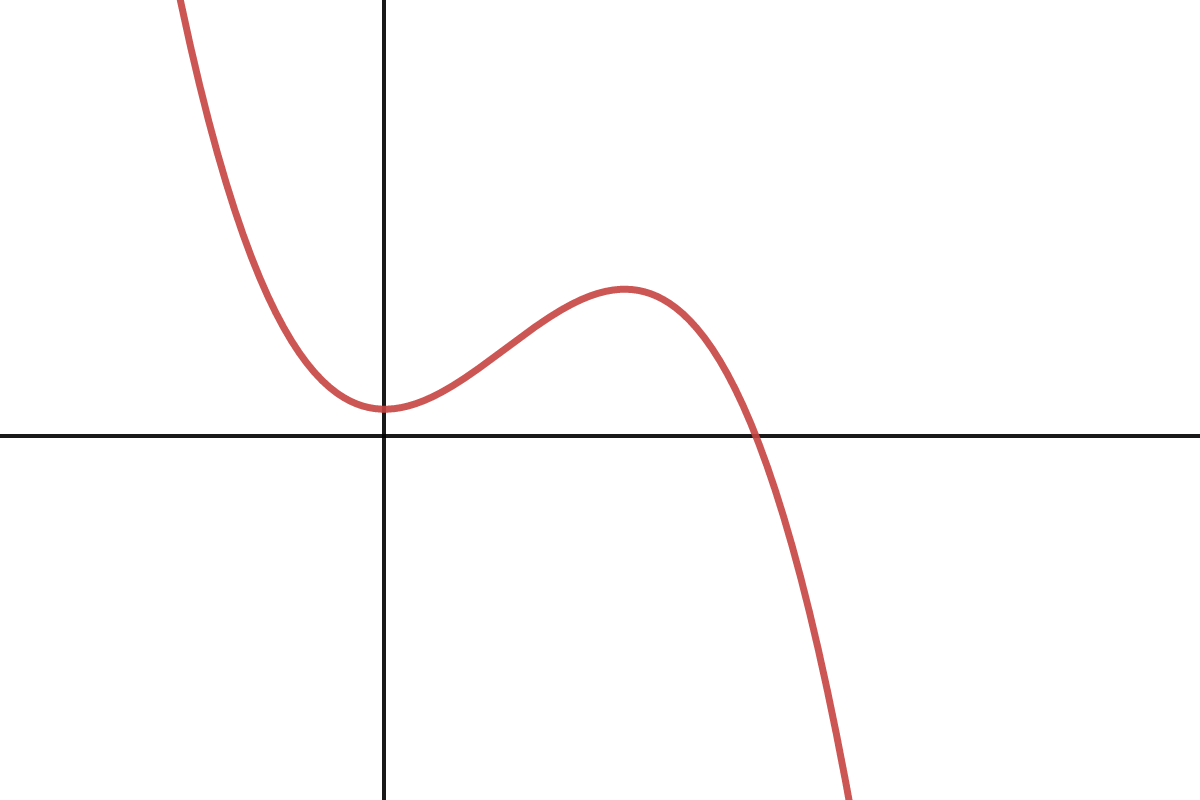
\includegraphics[height=0.25\textheight]{arclength1} \caption{Accessible interactive graph at \url{https://www.desmos.com/calculator/t8dz6vlmnz}}\label{arclength1}
\end{center}
\end{figure}

Let \(S\) be the arc length and \(\Delta S\) a short section of it, as illustrated in figure \ref{arclengthdx}.

\begin{figure}[!hptb]
\begin{center}
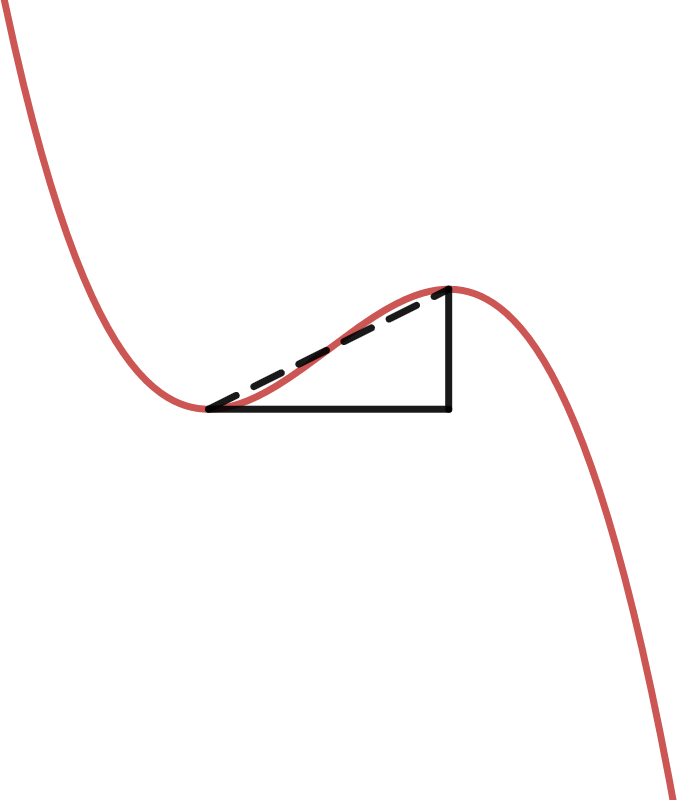
\includegraphics[height=0.25\textheight]{arclengthdx} \caption{Accessible interactive graph at \url{https://www.desmos.com/calculator/g5duc4kmfp}}\label{arclengthdx}
\end{center}
\end{figure}


\subsection{Derivation of Arc Length}

By Pythagoras' Theorem,
\[
\Delta S^2 \approx \Delta x^2+\Delta y^2
\qquad \Rightarrow\qquad
\left(\dfrac{\Delta S}{\Delta x}\right)^2 \approx 1+\left(\dfrac{\Delta y}{\Delta x}\right)^2
\]

As \(\Delta x\to0\) this becomes an identity
\[
\left(\dfrac{dS}{dx}\right)^2 = 1+\left(\dfrac{dy}{dx}\right)^2
\qquad\Rightarrow\qquad
\dfrac{dS}{dx} = \sqrt{1+\left(\dfrac{dy}{dx}\right)^2}
\]

The arclength between \(x=a\) and \(x=b\) is then
\[
\begin{aligned}
  S(a,b) &= \int_a^b\dfrac{dS}{dx}dx\\
  &= \int_a^b\sqrt{1+\left(\dfrac{dy}{dx}\right)^2}dx.
\end{aligned}
\]

\end{document}
